\subsection{Sơ đồ thực thể mối quan hệ}
\label{subsec:db_erd}

Schema có nhiều bảng cache nên một ERD duy nhất sẽ khó đọc trên khổ A4. Phần này chia ERD theo miền nghiệp vụ và chỉ giữ primary key, foreign key cùng các cột chính. Đường liền biểu diễn foreign key được khai báo trong PostgreSQL. Đường nét đứt biểu diễn liên hệ logic thông qua address, mint hoặc signature; các liên hệ này được kiểm soát tại service thay vì bằng foreign key.

\begin{figure}[H]
    \centering
    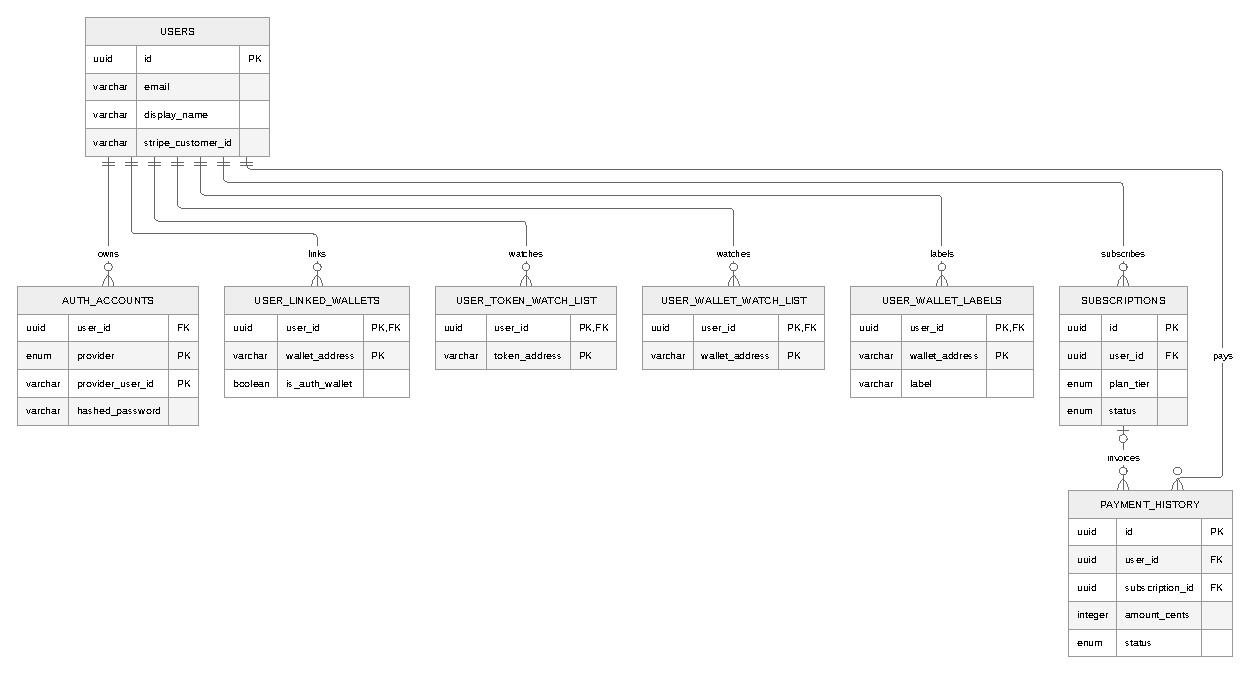
\includegraphics[width=\textwidth,height=0.78\textheight,keepaspectratio]{Chapter3/diagrams/identity-payment.pdf}
    \caption{ERD nhóm tài khoản và thanh toán}
    \label{fig:db_identity_payment}
\end{figure}

Hình~\ref{fig:db_identity_payment} thể hiện dữ liệu có tính sở hữu. Bảng \texttt{users} là gốc của dữ liệu xác thực, cấu hình cá nhân và thanh toán. Các bản ghi phụ thuộc người dùng được xóa theo quan hệ cascade; lịch sử thanh toán giữ được bản ghi khi subscription không còn tồn tại.

\begin{figure}[H]
    \centering
    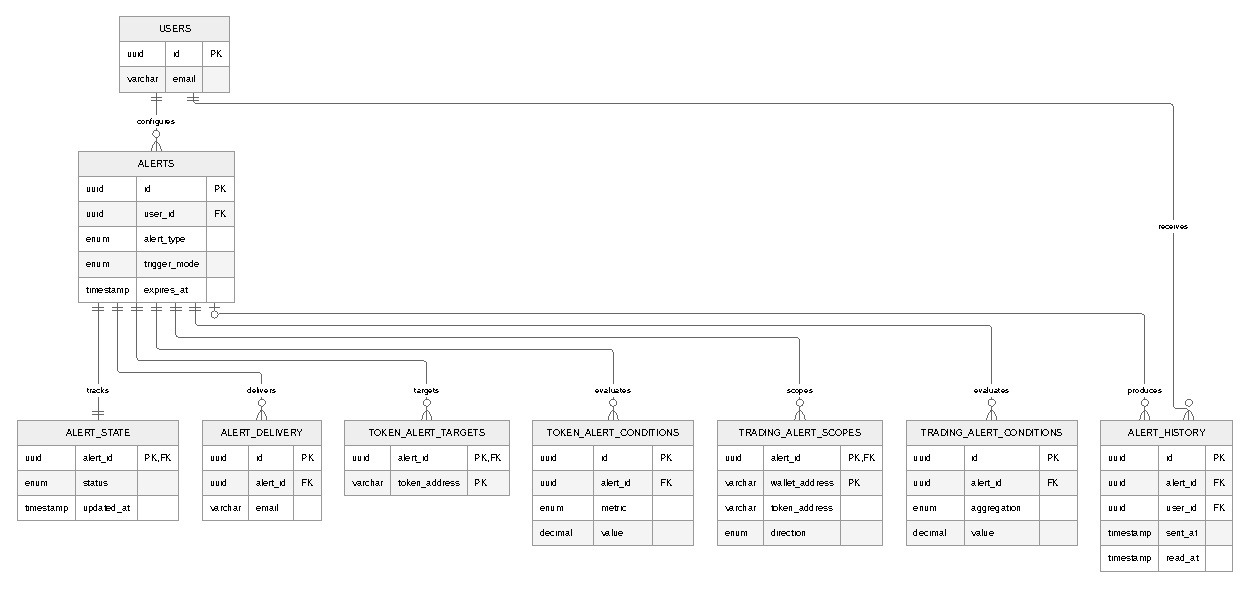
\includegraphics[width=\textwidth,height=0.78\textheight,keepaspectratio]{Chapter3/diagrams/alert-history.pdf}
    \caption{ERD nhóm cảnh báo và lịch sử cảnh báo}
    \label{fig:db_alert_history}
\end{figure}

Hình~\ref{fig:db_alert_history} tách định nghĩa cảnh báo khỏi trạng thái, delivery target và điều kiện kích hoạt. \texttt{alert\_history} lưu sự kiện đã phát sinh để hỗ trợ hiển thị lịch sử và trạng thái đã đọc.

\begin{figure}[H]
    \centering
    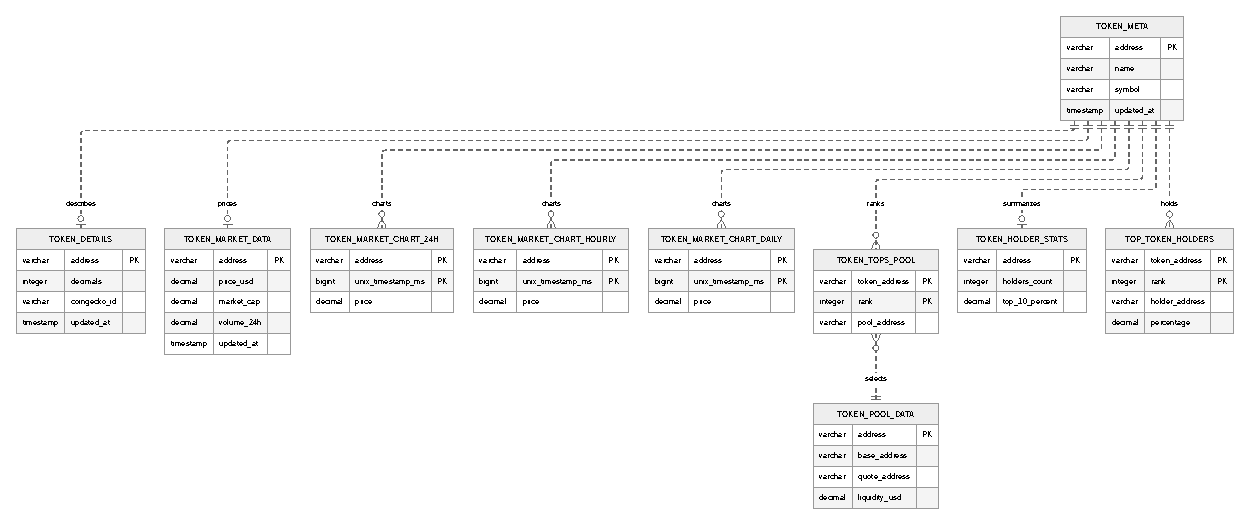
\includegraphics[width=\textwidth,height=0.78\textheight,keepaspectratio]{Chapter3/diagrams/token-market.pdf}
    \caption{ERD nhóm token và dữ liệu thị trường}
    \label{fig:db_token_market}
\end{figure}

Hình~\ref{fig:db_token_market} sử dụng \texttt{token\_meta} như điểm tham chiếu logic. Market snapshot và chart được cập nhật theo address và mốc thời gian. Pool và holder là các read model riêng, chỉ liên kết logic với token.

\begin{figure}[H]
    \centering
    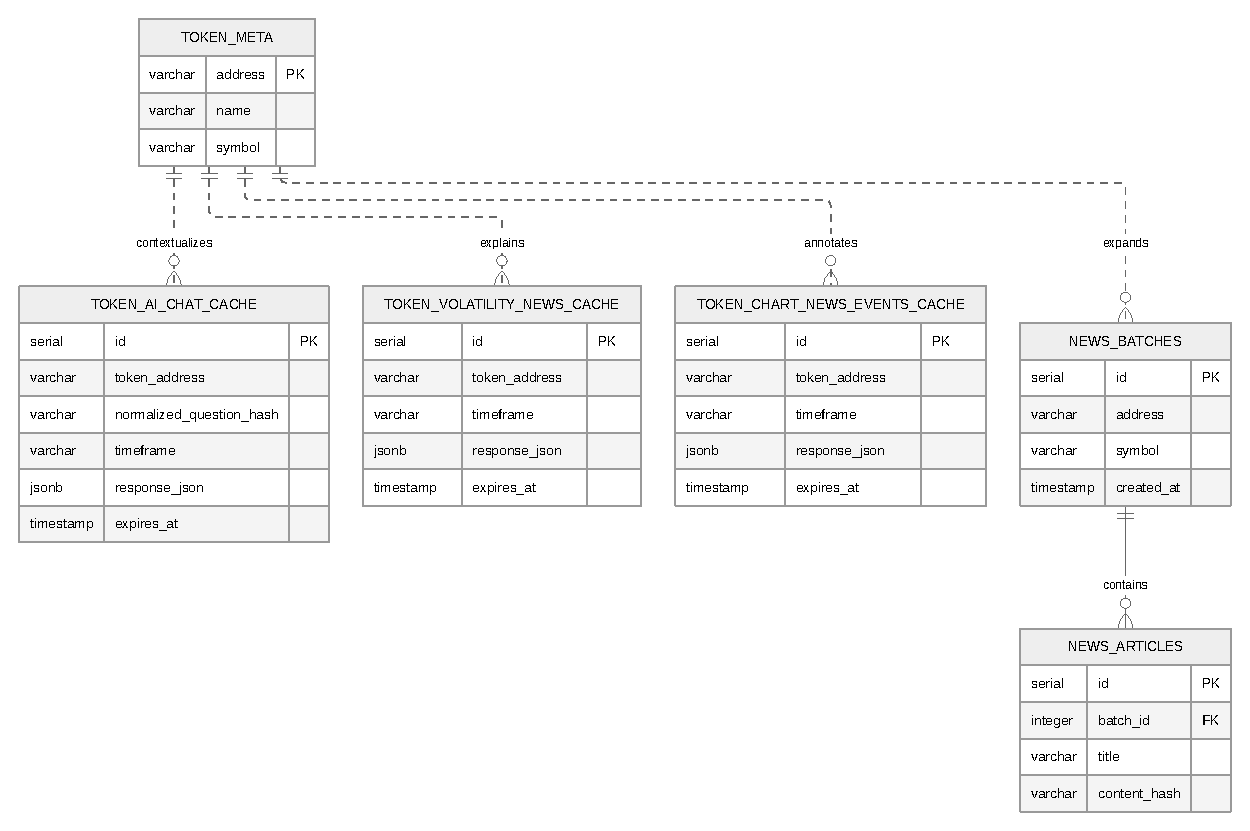
\includegraphics[width=\textwidth,height=0.78\textheight,keepaspectratio]{Chapter3/diagrams/token-content.pdf}
    \caption{ERD nhóm nội dung và AI cache theo token}
    \label{fig:db_token_content}
\end{figure}

Hình~\ref{fig:db_token_content} mô tả các cache phục vụ AI, news event và phần giải thích biến động. News batch có quan hệ khóa ngoại trực tiếp với article; các cache còn lại được ghép với token theo address.

\begin{figure}[H]
    \centering
    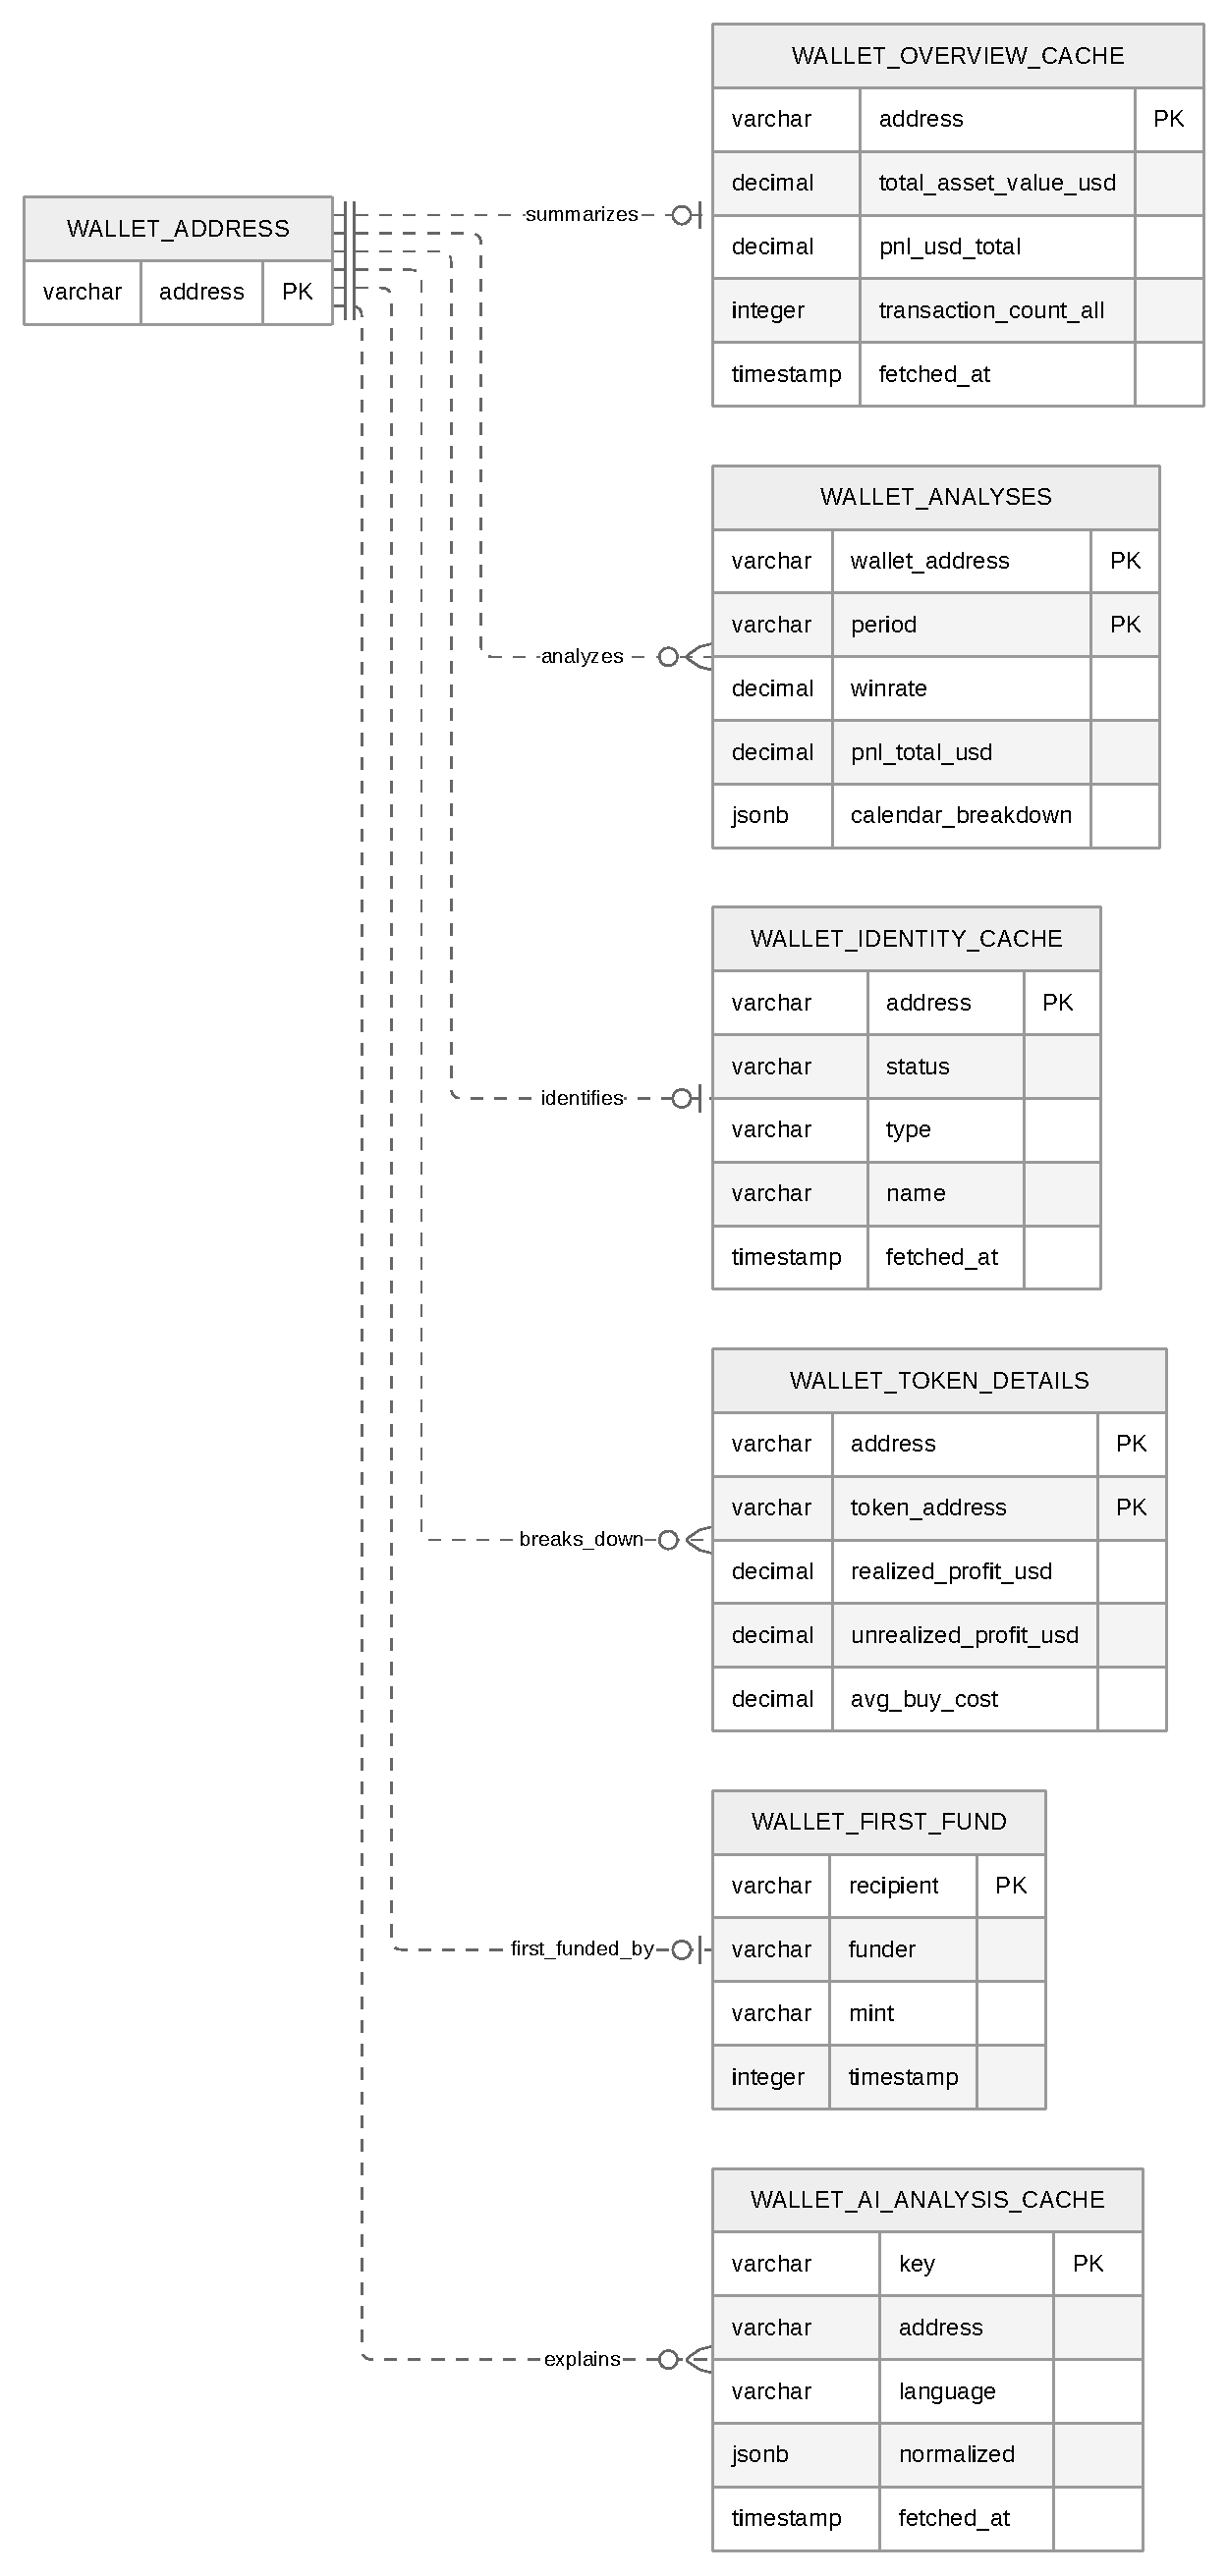
\includegraphics[width=\textwidth,height=0.78\textheight,keepaspectratio]{Chapter3/diagrams/wallet-analytics.pdf}
    \caption{ERD nhóm tổng quan và phân tích ví}
    \label{fig:db_wallet_analytics}
\end{figure}

Hình~\ref{fig:db_wallet_analytics} dùng \texttt{WALLET\_ADDRESS} như một thực thể logic, không phải bảng vật lý. \texttt{wallet\_overview\_cache} cung cấp bản tổng hợp cho trang overview. \texttt{wallet\_analyses} lưu kết quả Mobula theo ví và kỳ phân tích.

\begin{figure}[H]
    \centering
    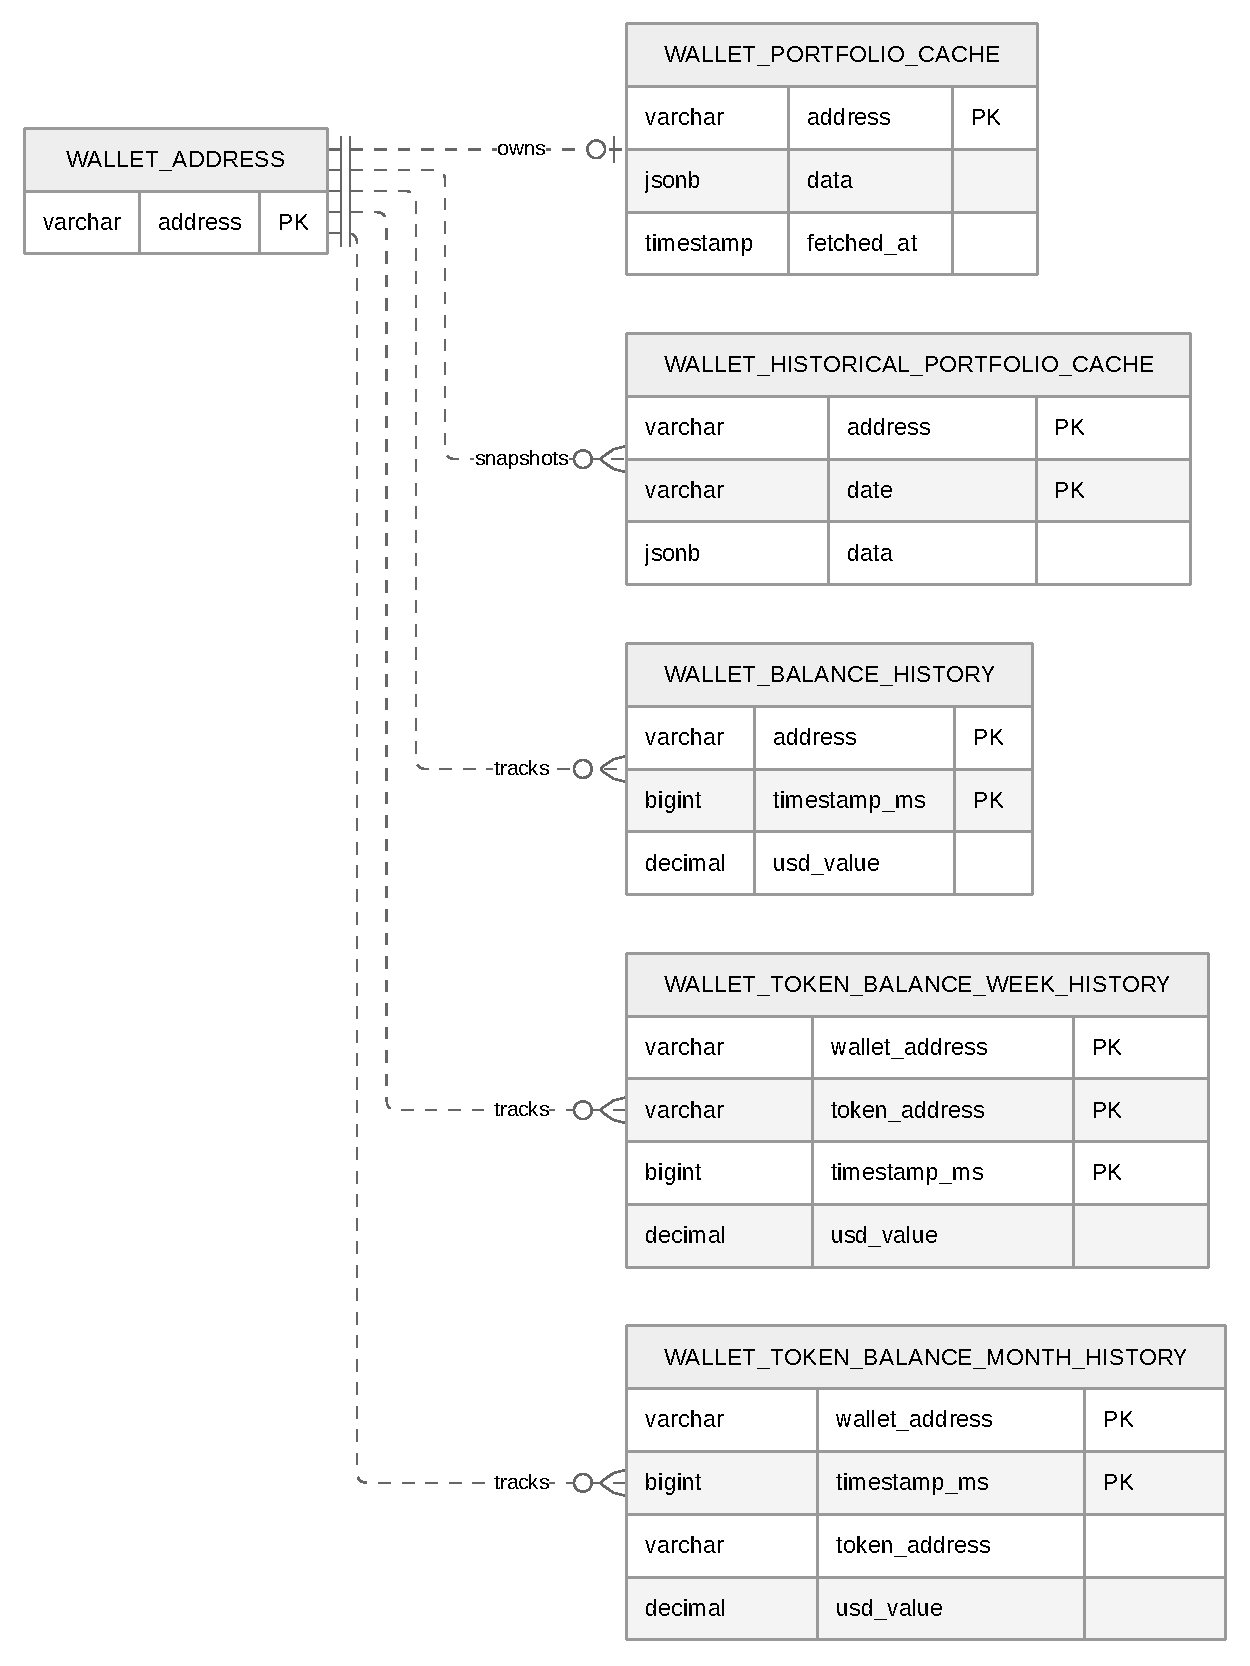
\includegraphics[width=\textwidth,height=0.78\textheight,keepaspectratio]{Chapter3/diagrams/wallet-portfolio-balance.pdf}
    \caption{ERD nhóm portfolio và lịch sử số dư}
    \label{fig:db_wallet_portfolio_balance}
\end{figure}

Hình~\ref{fig:db_wallet_portfolio_balance} phân biệt portfolio hiện tại, snapshot theo ngày, tổng giá trị ví theo thời gian và lịch sử số dư ở cấp token. Các bảng được ghép theo wallet address nhưng không phụ thuộc một bảng wallet vật lý.

\begin{figure}[H]
    \centering
    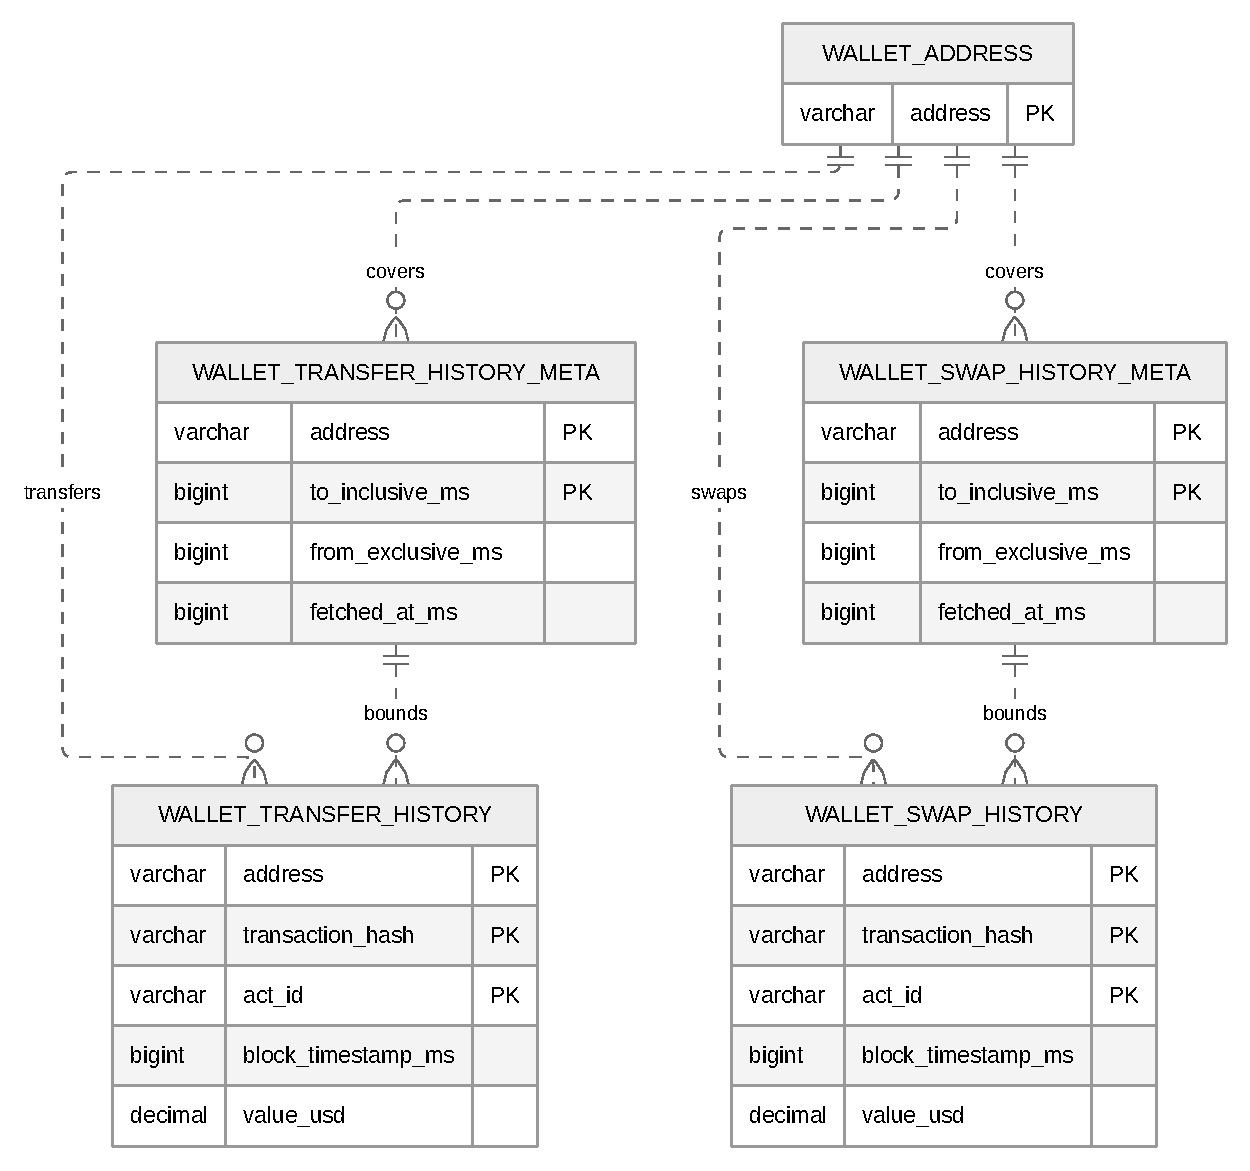
\includegraphics[width=\textwidth,height=0.78\textheight,keepaspectratio]{Chapter3/diagrams/wallet-history.pdf}
    \caption{ERD nhóm lịch sử transfer và swap}
    \label{fig:db_wallet_history}
\end{figure}

Hình~\ref{fig:db_wallet_history} tách dữ liệu lịch sử đã chuẩn hóa khỏi metadata coverage. Các bảng này phục vụ truy vấn phân trang và chỉ tải bổ sung những khoảng thời gian còn thiếu.

\begin{figure}[H]
    \centering
    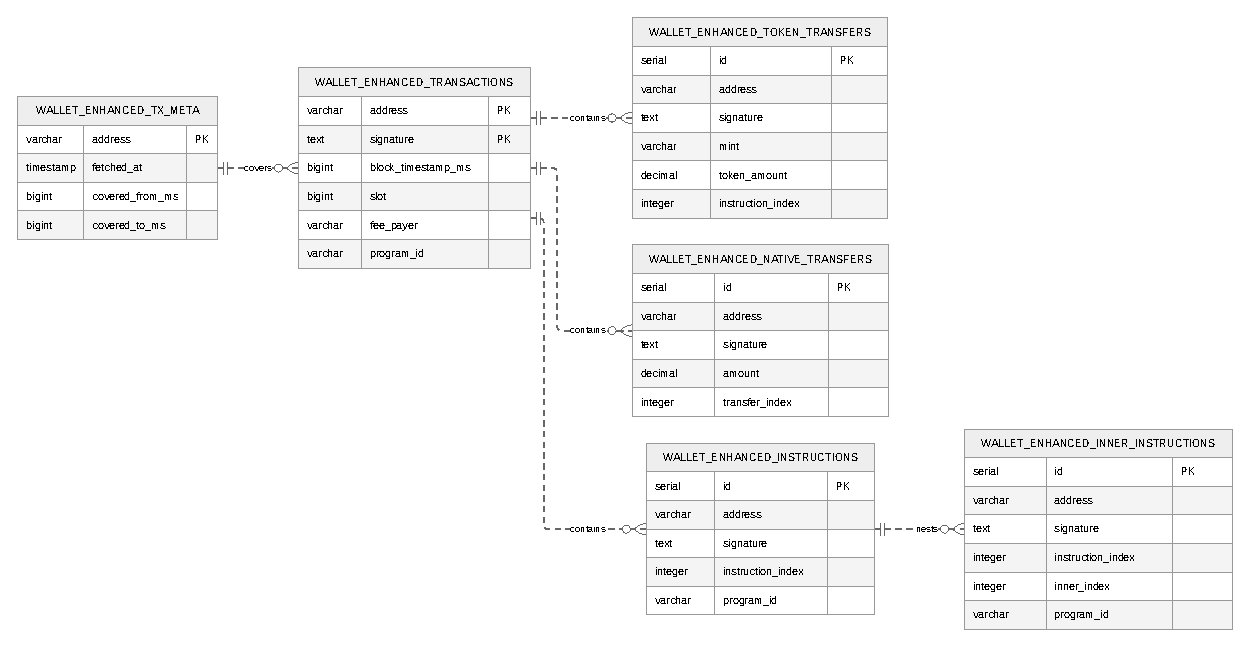
\includegraphics[width=\textwidth,height=0.78\textheight,keepaspectratio]{Chapter3/diagrams/enhanced-transaction-detail.pdf}
    \caption{ERD nhóm chi tiết giao dịch Helius}
    \label{fig:db_enhanced_transaction_detail}
\end{figure}

Hình~\ref{fig:db_enhanced_transaction_detail} mô tả read model chi tiết giao dịch. Bảng transaction cha được ghép với token transfer, native transfer và instruction bằng address cùng signature. Nhóm này phục vụ day activity, transaction detail và wallet analysis; nó không bị thay thế bởi transfer/swap history.
